\chapter{Problem statement}\label{ch:problem}
Currently there is no way of testing the full chain of devices towards and including an application to their limits without spending a lot of money on dedicated commercial load testing products.
Since today servers can be equipped with 40 and 100Gb/s Network Interface Cards (NICs), the OS and the application behind the NIC should be able to process the amount of traffic that comes in from the NIC.
Thus, with a commodity off-the-shelf server, it should be possible to test the infrastructure from client to server to see if it is able to handle the traffic to and from the server.
  
A wide variety of tools is available to generate traffic. Some of them offer an easy way of generating packets to be output by the interface and consume bandwidth. 
Others are able to setup TCP sessions to transfer data. But what tool is best used for specific application testing?   
Nikhef wants the ability to test hardware they might buy up to the OSI application layer (layer 7) if applicable. 
Until now they are not able to go beyond the transport layer (layer 4). 

\section{Session based}\label{sec:sessionbased}
When sending traffic over UDP, data gets dumped onto the link and is transported to the destination. If the destination is expecting data it will be processed.
When the destination does not know what to do with the data it will be discarded. 
TCP guarantees the delivery of the data as long as the session is alive between the end nodes. 
This is done by acknowledging received data and resending unacknowledged data. These acknowledgments need to be processed by the operating system. 
%When all the CPU's of a machine are busy generating packets the overhead of processing ACK messages will impact the maximum throughput of generating traffic. 
Other techniques like Flow control, Congestion control, and fast retransmission of packets ensure that data is delivered and offered to the higher layer protocol in the correct order. 
These techniques all require resource reservation at the client and the server, but also at stateful devices along the path between client and server. 
When a TCP session is created, memory is reserved by both the client and the server. In high speeds networks, the amount of reserved memory has to be relatively high in order to account for the unacknowledged packets in transit. 
Ubuntu 16.04 sets the resources reservation by default as follows:

\newpage

\begin{verbatim}
# maximum amount of read memory space in bytes
net.core.rmem_max = 8388608
# maximum amount of write memory space in bytes
net.core.wmem_max = 8388608
# amount of TCP read memory space in bytes (min, default, max)
net.ipv4.tcp_rmem = 131072 1048576 8388608
# amount of TCP write memory space in bytes (min, default, max)
net.ipv4.tcp_wmem = 131072 1048576 8388608
\end{verbatim}  

The default TCP memory allocation is chosen for the first sessions. But when more sessions are opened up the amount of allocated memory per session drops to the minimum amount to save possibly unused resources. 
Unfinished sessions keep this memory allocated. 
When the amount of new sessions is higher than the amount of sessions that get closed due to a time-out, server resources are depleted.
These memory usage settings are applicable for kernel based applications and can be tuned if one wishes to do so. 
The memory settings are not changed during this research since the correct settings for reaching the best performance depends on the application.
The kernel settings are default for every tool discussed in chapter \ref{sec:tools}.  

When it comes to layer 7 protocols like HTTP, more resources need to be reserved. HTTP sessions, HTTP state and application state need to be saved. Get requests need to be processed, a response needs to be generated and sent over the session to the user. Normally a web server will cache files that are requested for a specific time using up valuable memory. Hosting a dynamic web page requires the web server to generate the page on request which makes the CPU utilization higher than just hosting a static web site. 

\section{Specifications}\label{sec:specifications}
For the design of the tests and the interpretation of the results, specific technical constraints in the 'real world' operating environment and several key implementation parameters are important for this project.

\paragraph{Throughput}\label{par:throughput}\mbox{}\\
Throughput is the most significant value for generating load: how to best utilize the total capacity of a link. When using TCP the header causes 12 bytes more overhead in comparison to a UDP header (a UDP header is 8 bytes).

\paragraph{Packet size}\label{par:packetsize}\mbox{}\\
Ethernet is used during this research, therefore all references to packet sizes are based on Ethernet standards\cite{ethernet_frame_2017} with IP and TCP headers included.
Due to collision detection the minimum payload inside an Ethernet frame is 46 bytes.
The Ethernet frame and the payload combined have a minimum size of 64 bytes. 
A VLAN tag is excluded which adds 4 bytes.
A packet is always preceded with a 8 byte preamble.
An Inter Frame Gap between the packets is used to separate the packets. This is a 12 byte gap. 
This makes a total of at least 88 bytes of data from the beginning of a packet to the beginning of a new packet. Figure \ref{fig:juniperethernetframe} gives a representation of an Ethernet packet. 

\begin{figure}[H]
  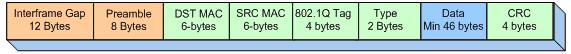
\includegraphics[scale=1]{images/ethernetframe.jpg}
  \caption{Representation of an Ethernet frame used during this report.}
  \label{fig:juniperethernetframe}
\end{figure}

\paragraph{Packets per second}\label{par:pps}\mbox{}\\
When a link has a speed of 40Gb/s and packets have a minimum size of 88bytes (which includes the inter frame gap, the preamble the data link frame and a VLAN tag) a maximum of 56.8 Million packets per second (Mpps) can be transferred over the link in one direction. When using a 100Gb/s line the theoretical maximum is 142 Mpps.   

\paragraph{Sessions}\label{par:sessions}\mbox{}\\
A TCP session is a unique tuple of source IP, destination IP, source port and destination port. An established session may involve more than one message in each direction.
The amount of sessions per second is a determining factor for the availability of services behind firewalls. A firewall needs to keep track of the states of the sessions from source to destination. 
When new sessions to a server are opened, the firewall has to process them according to the rule base. When a session is approved, most vendors move it to fast-path processing. 
This is a table with accepted sessions, allowing traffic in the same session to be handled in hardware. This means that only the first packet of a new session is handled in the slow-path and the limitations of a firewall can be found in the amount of new sessions per second.

\paragraph{Application specific traffic}\mbox{} \\
According to Sandvine\cite{phenomena_2017},(a global communications solutions service provider that published bi-annual traffic baseline reports), around 70\% of the traffic is streaming audio and video. In second place is web browsing and third are marketplace solutions. A lot of on-line services are accessed through a web page. 
Since web browsing is in second place it is interesting to look at HTTP traffic as a layer 7 protocol. 

\paragraph{Packet size}\label{par:packetsize}\mbox{}\\
According to Murray et all. \cite{murray2012state}  in 2012, 99\% of the traffic inside a corporate network has an MTU size of maximum 1500 bytes. When using Jumbo packets\cite{alliance_2017} (Best practice is an MTU of 9000 bytes towards clients\cite{jet}) the amount of overhead is less because more data can go into on packet. 
More data inside a packet results in less packets. Therefore, less system overhead during the transfer of data. 
Jumbo packets can help when large amounts of data need to be transfered.  
Jumbo packets are not used during the project unless mentioned otherwise during a test.

\newpage
\section{Research question}\label{sec:researchquestion}
The problem statement and the specifications lead to the following research question.

\begin{center}
\textit{What is needed to perform high bandwidth session based throughput tests and how to go beyond pure network infrastructure testing?} \\
\end{center}
The term "high bandwidth" references to at least 40Gb/s. \\
The term "session based" references to TCP traffic. \\

